\documentclass[12pt]{article}

\usepackage{amsmath}
\usepackage{graphicx}
\usepackage{tabularx}
\usepackage{natbib}
\usepackage{todonotes}
\usepackage{amssymb}
\usepackage{amsfonts}
\usepackage{amsthm}
\usepackage{mdframed}
\usepackage{float}
\usepackage[labelfont=bf]{caption}
% To do commands
\newcommand{\slava}[1]{\todo[color=blue!40]{#1}}
\newcommand{\trish}[1]{\todo[color=green!20]{#1}}

\title{Master's Proposal}
\author{Slava Nikitin}
\date{\today}

\begin{document}
\maketitle

\tableofcontents

%%%%%%%%%%%%%%%%%%%%%%%%%%%%%%%%%%%%%%%%%%%%%%%%%%%%%%%
\section{Introduction}
	The basic fact that underpins this proposal is that every statistical model is a simplification, thus it is limited in inferences it supports. If questions motivating research go beyond the inferential capacity of a model, then it is natural to construct a new one. The question I want to ask is whether and in what way psychological processes responsible for simple decision making are coordinated across trials to perform two-choice tasks (e.g. does the stimulus move right or left?). The answer to this question will enrich understanding of sequential properties of cognitive processing.

	A long history of investigating simple decisions points to duration of encoding stimulus features, rate of information uptake, level of caution, decision bias and response execution duration as key psychological parameters driving performance \citep{Sto1960,Vic1979,TowAsh1983,Luc1986,BogRaf2006}. Coordinated adjustments of psychological processes would be present if sensible tradeoffs between parameters took place to maintain a certain level of speed-accuracy. For example, assuming that all key processes are involved in controlling the tradeoff between speed and accuracy, then to raise accuracy a sensibly designed cognitive system would increase time for stimulus processing, increase rate of information uptake, raise level of caution, remove decision bias and prolong response execution time. Tendency towards faster responses would flip the pattern. Presence of tradeoffs would imply statistical dependencies among parameters.

	However, in applications of prominent models of simple decisions, it is common to assume that psychological parameters fluctuate across trials in a mutually independent manner \citep{RatTue2002,UshMcc2001,BroHea2008}. The implication of the independence assumption is that there is no general, long-term coordination of processes. Instead, processes could be adjusted arbitrarily through selective experimental manipulations \citep{VosAnd2004}. For example, giving instructions to participants to emphasize speed or accuracy would affect only the caution parameter \citep{RatMck2008,Wag2009,VanTue2007,VanTue2011,RaeHea2014}. Change in caution would not correlate with any other parameter.
    
	Also, the lack of general coordination is also consistent with coordinated adjustment, stretching short sequences of trials. In this case, different sequences would have different tradeoffs leading to long run independence. For example, post error slowing is a short-term phenomenon that arises from participants monitoring their performance and adjusting their processing to maintain a relatively constant level of accuracy \citep{VanMal2004}. While a common suggestion is that slowing is solely due to caution increase, a recent study comparing old and young adults showed evidence for coordinated changes \citep{DutFor2013}. Model-based analysis concluded that rate of uptake decreased, caution increased and nondecision time increased. However, the post error pattern of parameter adjustments may not represent a general trend of coordination, and change over the next few trials.
    
	While both selective influence of processes and short-term dependencies of post error slowing support the notion that there is no general coordination of cognitive processes, I would like to test it more directly. A common approach to answering questions about cognitive processing is to build a mathematical model. Statistically, dependencies imply associations among parameters that are assumed to vary across trials. The dominant class of cognitive process models developed to account for simple decision making lacks structure to make inferences about process dependencies \citep{SmiRat2004}. Thus, answering the question about process coordination requires a new statistical model.
    
	I propose to take an empirically well tested model of simple decisions and add an association structure that shapes how parameters fluctuate across trials. The model will enable testing the assumption of independent parameters that implies no general coordination of processes and measuring whatever associations that could be present. 
    
	The proposal will unfold in the following way. First, I discuss why the cognitive process model is an approach I take to answer the question about process coordination and dependencies. Then, to provide context, I will introduce the simple decision making phenomenon and discuss how it is studied in the laboratory. Third, I will introduce sequential sampling framework for modeling simple decisions, and focus on the Ratcliff diffusion model, a prominent sequential sampling model that can account for main features of experimental data. Fourth, I will describe specific problems in developing models with association structure and methodology for solving them. Finally, I will define three studies that should provide answers to the posed problems.

%%%%%%%%%%%%%%%%%%%%%%%%%%%%%%%%%%%%%%%%%%%%%%%%%%%%%%%
\subsection{Development of Cognitive Models}
Psychology has as one of its chief aims identification of the cognitive architecture that generates the rich repertoire of human behavior and is sensitive to many environmental variables \citep{AndBot2004,And2007}. More specifically, a psychologist wants to learn about the number, temporal arrangement, individual characteristics and interactions of elementary processes and representations. A fundamental obstacle is that cognition is not directly observable. From the perspective of systems identification, the study of human cognition is an instance of a black box problem \citep{Lju1999, Lju2010}. Working on a black box problem, a researcher only has direct information about the system’s input and output, but lacks direct access to internal processes transforming inputs into outputs. The problem then is how to identify internal processes from known combinations of inputs and outputs, that is how to uncover the human cognitive architecture from information about overt behavior taking place in some environment. 

	An approach to providing an approximate solution to the black box problem is construction of competing mathematical models that can be tested against data using statistical methods \citep{Lju1999,Lju2010,CasBer2002,GelCar2013}. A model that best balances parsimony, fit to empirical regularities and interpretability can be taken as an approximate solution, and provide valuable insights about internal processes. This approach fits well with psychological phenomena because it is often easy to come up with several, categorically different conjectures about the underlying cognitive processing \citep{TowAsh1983}. The best way to ensure coherency of conjectures about cognition, and improve their falsifiability, is to formalize them in mathematical models \citep{BusDie2010,LewFar2010,LeeWag2014}. For instance, a model that can predict a power relation between time and memory retention is easier to falsify than a verbal account that only makes ordinal predictions \citep{CavMyu2013}. Ultimately, the goal is to use models of cognition to draw insights about elementary processes and how they change under experimental manipulations, across individuals and groups.
    
	A paradigm case of modeling cognition is signal detection theory \citep{MacCre2004}. The original phenomenon motivating development of signal detection models was human ability to make decisions with distorted sensory stimuli. This phenomenon can be studied experimentally using a computerized task. For example, during the auditory signal detection task an observer is presented with a sequence of stimuli drawn either from a “Signal” distribution representing a tone combined with white noise, or a “Noise” distribution representing white noise. On each trial, an observer has to respond “Yes” if he decides the stimulus belongs to the “Signal” distribution and “No” otherwise. Under these conditions, a researcher knows which class each presented stimulus belongs to and observes a sequences of responses, typically summarized as hit rate (proportion of true positives) and false alarm rate (proportion of false positives). The problem is to learn about cognitive processes involved in transforming stimulus information into responses from the generated data.
    
	Signal detection models are probabilistic models that specify how elementary cognitive processes operate on information contained in external stimulus to produce hits and false alarms \citep{MacCre2004,LeeWag2014}. The basic idea is that signal detection can be formalized as a random decision procedure:
    
\begin{enumerate}
\item Sample randomly a stimulus from either a “Signal” or “Noise” class
\item Sample randomly a strength value given a class of the stimulus
\item If the strength value is greater than or equal to a threshold then respond “Yes”, otherwise respond “No”
\item Repeat steps $1$--$3$ for N trials
\end{enumerate}
Mathematically, let a random variable $C \in \{0, 1\}$  represent a stimulus randomly drawn either from a “Noise” class or “Signal” class, respectively. The probability mass function of $C$ is determined by the experimenter. In response to the sampled stimulus an internal representation of strength value, represented by a random variable $X \in \mathbb{R}$, is generated. $X$ conditioned on stimulus class is normally distributed with class specific mean and variance parameters: 

\begin{align}\nonumber
X \mid C = 1 \sim \mathcal{N}(\mu_s, \sigma_s^2)\\
X \mid C = 0 \sim \mathcal{N}(\mu_n, \sigma_n^2)
\end{align}

Finally, let $\tau$ represent a threshold which is defined as the distance from a point ${\frac{\mu_s - \mu_n}{2}}$,   where the two normal probability density functions intersect. Then a random variable 

\begin{equation}
R = \left\{
	\begin{array}{l l}
     1, & X \geq \tau\\
     0, & X < \tau
     \end{array}\right.
\end{equation}
represents a “Yes” or “No” response, respectively. 

	This version of the model has five free parameters, but it usually gets simplified by restricting $\mu_n = 0$ and $\sigma_n^2 = 1$. The other three parameters remain free and quantify central features of processing supporting signal detection. The sensitivity parameter, $d' = \mu_s - \mu_n = \mu_s$, quantifies how well the encoding process separates “Noise” from “Signal” stimuli. The threshold $\tau$ represents the decision criterion and the ratio of variances $\frac{\sigma_n^2}{\sigma_s^2} = \frac{1}{\sigma_s^2}$ between “Noise” and “Signal” distributions characterizes relative noise in representations. These three parameters drive the predicted pattern of responses. 
    
	To begin testing a specified cognitive model one needs to derive, or be able to simulate, predictions for performance data. In the signal detection case, the random mechanism specified above, and an additional assumption that all responses during an experiment are mutually independent, allow for an analytical derivation of a probability mass function parameterized by the three free parameters.  The derived model for $Y_h = 0, 1, \ldots, N_h$ hits and $Y_{fa} = 0, 1, \ldots, N_{fa}$  false alarms for a given participant is a product of two binomial mass functions    
    
\begin{gather}
f(y_h, y_{fa} \mid p_h, p_{fa}, N_h, N_{fa}) = \nonumber \\
\binom{N_h}{y_h}p_h^{y_h}(1 - p_{h})^{N_h - y_h}
\binom{N_{fa}}{y_{fa}}p_{fa}^{y_{fa}}(1 - p_{fa})^{N_{fa} - y_{fa}}
\end{gather}
with unknown probabilities as functions of cognitive parameters
\begin{align}\nonumber
p_h = P(R = 1 \mid C = 1) = \Phi(\frac{0.5d' + \tau}{\sigma_s}) \nonumber \\
p_{fa} = P(R = 1 \mid C = 0) = \Phi(-0.5d' - \tau),
\end{align}
where $\Phi( )$ is a normal cumulative distribution function.
    
	Once a statistical model relating cognitive parameters and data is specified for a given theory, one can use a rich body of statistical methods to explore its predictions via simulations, to estimate its free parameters from data, to compare and select from competing models of a cognitive processing involved in a given task \citep{Ber1997,CasBer2002,GelCar2013}. Connecting the signal detection model to performance data enables a researcher to make a range of inferences about cognitive processes involved in signal detection. For instance, it is possible to test goodness of fit of a model with $\sigma_s^2 = 1$ against a model where $\sigma_s^2$ is a free parameter to determine noise properties of stimulus representation. However, the range of possible inferences is limited, so the specified model cannot say anything about adaptations of the representations or motor processing. It would require a new model to address additional questions about signal detection. 

%%%%%%%%%%%%%%%%%%%%%%%%%%%%%%%%%%%%%%%%%%%%%%%%%%%%%%%
\subsection{Phenomenon of Simple Decision Making}
	Developing new cognitive process models is a central tool for learning about the human cognitive architecture \citep{BusDie2010,LewFar2010,LeeWag2014}. The main problem addressed in this thesis is a generalization of a well-established cognitive process model of simple decision making in a way that enriches potential insights about process interactions drawn from behavioral data. Before discussing models, I will briefly delineate the simple decision making problem motivating models of interest, and discuss experimental designs used to collect empirical regularities against which the models can be tested.
    
	The psychological problem of interest can be posed in this way: how does a human observer, in a short amount of time and with above chance accuracy, choose, according to a preset rule, among a discrete set of responses using confusable sensory stimuli? Computationally, the problem is to map stimulus information into action \citep{Vic1979,BogRaf2006}. A variety of tasks could be constructed to study underlying processes by varying the sensory modality, the number of choices, the number of stimulus attributes relevant to the decision, response modality and whether a participant or an experimenter controls decision timing. I will concentrate on participant-controlled two-choice tasks, driven by a single feature of a stimulus. These tasks have been extensively used in experiments and for developing cognitive models of simple decision making, thus they make a solid starting point for developing a new model \citep{Luc1986,RatSmi2004,RatMck2008,Wag2009}.
    
	An example of a two-choice task is a numerocity task \citep{RatLov2012}. On a given trial, two clouds of points consisting anywhere from a few dots to hundreds are presented simultaneously. The relative number of dots is deliberately picked to be similar to induce uncertainty about the correct decision, and create imperfect performance. An observer has to make a decision according to a rule such as “pick the cloud with the larger number of points” within a short period of time, ranging roughly from 250 to 1000 milliseconds \citep{RatLov2012}. 
    
	Other two-choice paradigms include deciding in which direction dots are moving, deciding whether a distorted character is an English letter, deciding which pixelated square is brighter, and deciding whether a word was studied before or not \citep{SmiRat2004,RatSmi2004,RatRou1998,PerVan2002}. The data generated by these tasks often include response times and responses under a variety of robust experimental manipulations \citep{Luc1986}. For example, when deciding whether a distorted character is an English letter a researcher could vary level of distortion, probabilities of English and non-English letters, and instructions emphasizing either speed or accuracy in decisions. Empirical patterns arising from these manipulations can be repeatedly detected in response time distributions for correct and error responses, response proportions, and relations between response proportions and corresponding mean response times. In total, two-choice tasks tap into a relatively tractable psychological problem, and provide a rich empirical record to test abstract cognitive process models.
    
%%%%%%%%%%%%%%%%%%%%%%%%%%%%%%%%%%%%%%%%%%%%%%%%%%%%%%%%%%%%%%%%%
\subsection{Sequential Sampling Models}
	A common approach to modeling cognitive processing underlying two-choice tasks is to decompose it into processes of encoding of stimulus features, response selection based on a relevant stimulus feature and motor execution. A cognitive process model for these tasks should make sufficient assumptions about these processes to predict patterns in performance data. A delicate balance has to be struck between what details to include and what details to exclude because it will determine generalizability of models across two-choice tasks. For instance, including details about how lexical information is accessed in memory to direct response selection will make a model inapplicable to brightness discrimination. The dominant approach to this balancing problem is sequential sampling framework. 
    
	A fundamental theoretical assumption of sequential sampling framework is that the same general decision process operates across all two-choice tasks. Then, a generalizable model should provide a detailed account of the decision process while making few assumptions about the stimulus encoding and motor processing. Over the last $~50$ years, many models of this type have been developed, and some of its most successful members can explain all the major patterns in the response time and response data, under a variety of experimental conditions and tasks \citep{Sto1960,Rat1978,RatTue2002,Smi1995,UshMcc2001,BroHea2008}. Some models have also been used for predicting firing rates in neural populations representing choices \citep{RatChe2003,RatHas2011,SmiRat2004,Bog2007}, but I will concentrate on performance data.
    
	The underlying principle of sequential sampling models is that when an observer is tasked with selecting the correct response, in limited time based on noisy stimulus, he samples and integrates information from the relevant stimulus feature until one of two decision thresholds is reached \citep{Sto1960,Edw1965,Pik1973,Rat1978,UshMcc2001,RatSmi2004,SmiRat2004,RatMck2008,Wag2009,Luc1986,TowAsh1983,BogRaf2006}. By controlling his thresholds, the observer can balance the trade-off between speed and accuracy of response \citep{BogWag2010}. Bounded accumulation of information naturally provides predictions of performance data collected during two-choice tasks. Accumulation times vary from run to run to produce distributions of response time and which threshold is reached first determines the response.
    
	Given the sequential sampling principle, any concrete model of simple decisions makes detailed assumptions about the nature of sampled information, temporal structure of sampling, stopping rule and sources of randomness \citep{RatSmi2004,BogRaf2006,TeoUsh2013}. Combinations of modeling assumptions generate the range of possible sequential sampling models. For example, the sampled information can consist of discrete or continuous packets. The size of the packets may be fixed or variable. The accumulation of information packets may happen at fixed or variable discrete time points, or continuously. The stopping rule may be absolute, in which case accumulation stops when evidence in favor of one of the choices reaches a threshold, regardless of the amount of evidence favoring the alternative. In contrast, the relative rule requires that evidence favoring one of the choices has to exceed the other by some amount.
    
	Examples of sequential sampling models include a random walk model that stops accumulation of discrete packets of randomly varying information over discrete time according to a relative rule \citep{Lam1968}, a Poisson counter model that continuously accumulates discrete, fixed information packets until evidence for either of the choices reaches a threshold \citep{Lab1962}, and a Wiener diffusion model that describes accumulation of continuous packets in continuous time until a relative threshold \citep{Rat1978}. I will concentrate on an empirically successful Ratcliff diffusion model \citep{RatTue2002} as a base for incorporating assumptions about process associations. 
    
%%%%%%%%%%%%%%%%%%%%%%%%%%%%%%%%%%%%%%%%%%%%%%%%%%%%%%%%%%%%%%%%%
\subsection{Ratcliff Diffusion Model}
	The Ratcliff diffusion model is a variant of the Wiener diffusion model (Laming, 1968; Link and Heath, 1975; Ratcliff 1978; Ratcliff and Rouder, 1998; Ratcliff and Tuerlinckx 2002). I concentrate on this model because of its long development and examination (Ratcliff, 1978; Ratcliff and Rouder, 1998; Ratcliff, 2002; Ratcliff and Tuerlinckx, 2002; Ratcliff, 2013), and successful testing against a wide range of experimental data (Ratcliff and McKoon, 2008; Wagenmakers, 2009). As with all sequential sampling models, predictions about performance data are primarily implications of the structure of the information integration process formalized in the language of stochastic processes (Ross 2014; Karlin and Taylor, 1975, 1981).
    
	Underlying the Ratcliff model is a continuous time, continuous state space stochastic process that begins at some starting point and evolves until one of two absorbing boundaries. Formally, it is an uncountable, ordered collection of univariate random variables
    
\begin{equation}
\{X(t); t \geq 0\}
\end{equation}
with the index set being the positive real numbers. In psychological application, the state space is defined by the interval $[0, \alpha]$, where $\alpha > 0$. There several ways of fully defining the Wiener process. One way is to describe properties of points and increments of the process. The two-boundary Wiener process satisfies
\begin{enumerate}
\item $X(t)$ is an almost surely continuous function
\item $X(0) = \zeta$
\item $X(t) \sim \mathcal{N}(\delta t, \sigma^2 t)$
\item Stationary and independent increments
\end{enumerate}
In contrast, one can consider the evolution of the Wiener process, formalized by the stochastic differential equation

\begin{equation}
dX(t) = \delta t + \sigma dW(t)
\end{equation}
where $W(t)$  is a standard Wiener process with points distributed as standard normal variates. The Wiener process $X(t)$ is the solution to the equation.

	In addition to the mathematical assumptions, the Ratcliff diffusion model also provides linking assumptions that interpret parameters of the process in cognitive terms. Boundaries of the state space, 0 and $\alpha$, represent the amount of evidence needed for each response, i.e. decision thresholds. The lower bound could represent the error response, or one of the responses, say “Noise” in the auditory signal detection experiment. Similarly, the upper bound could represent the correct response, or “Signal” response in the auditory signal detection experiment. The separation between boundaries quantifies caution because larger separation implies more information is required before making a response. 
    
	The starting point of the process, $\zeta$, represents the initial amount of information from which the accumulation process begins. The initial information satisfies $0 < \zeta < \alpha$. The level of initial information represents the bias an observer may have towards one of the responses. Based on this interpretation the process can be reparameterized by replacing starting point with bias

\begin{equation}
\beta = \frac{\zeta}{\alpha}
\end{equation} 
 
	The accumulation process is controlled by two parameters. The drift rate coefficient $\delta \in \mathbb{R}$  is the infinitesimal mean change in the state of the diffusion process, and is interpreted to measure the speed of information uptake. The diffusion coefficient $\sigma^2 > 0$  stands for the infinitesimal variation in the state of the diffusion process, and describes the amount of noise in the decision process. Mathematically, $\sigma^2$ works as a scaling parameter. For example, if $\sigma^2$ is rescaled by a factor $c > 0$, then the process makes identical predictions if all the other parameters are rescaled by $c$. I will take the usual assumption $\sigma^2 = 0.1$.
    
    The two-boundary Wiener process provides a straightforward way to predict performance data. During a single run, a Wiener process will start at $\zeta$ and take some random time to reach one of the boundaries before it stops. Let $T^d > 0$ be the random time taken to first pass a boundary and $R \in {0, 1}$ be the random boundary passed. Then, the probability of reaching the upper bound 
\begin{equation}
P(R = 1) = \frac{\operatorname{exp}(\frac{-2\delta \zeta}{\sigma^2})-1}{\operatorname{exp}(\frac{-2\delta \alpha}{\sigma^2})-1}
\end{equation}
quantifies the probability of the corresponding response, say a correct response. The joint probability density function of $T^d$ and $R$

\begin{gather}
\label{eq:wd}
f(t^d, r \mid \alpha, \delta, \zeta, \sigma^2) = \nonumber \\
\begin{cases}
\frac{\pi\sigma^2}{\alpha^2}\operatorname{exp}(-\frac{\delta\zeta}{\sigma^2}-\frac{\delta^2t^d}{2\sigma^2})\sum_{k=1}^\infty{k\operatorname{exp}(\frac{-k^2\pi^2\sigma^2t^d}{2\alpha^2})\operatorname{sin}(\frac{k\pi\zeta}{\alpha})}, & r = 0\\
\frac{\pi\sigma^2}{\alpha^2}\operatorname{exp}(\frac{\delta(\alpha - \zeta)}{\sigma^2}-\frac{\delta^2t^d}{2\sigma^2})\sum_{k=1}^\infty{k\operatorname{exp}(\frac{-k^2\pi^2\sigma^2t^d}{2\alpha^2})\operatorname{sin}(\frac{k\pi(\alpha - \zeta)}{\alpha})}, & r = 1
\end{cases}
\end{gather}
However, $T^d$ only counts the decision time. To fully connect the Wiener process to performance data, the model requires assumptions about the perceptual and motor processes surrounding the information integration stage.

	Common decomposition of two-choice tasks implies that before information sampling can begin, the sensory stimulus has to be transduced and its features encoded. When the accumulation reaches one of the thresholds, the observer has to organize and execute a motor response for their decision to be registered. The details of such perceptual and motor processing are typically not specified (but see \citet{SmiRat2009}), but their time is captured by a single parameter $\tau^er$. Then, response time
\begin{equation}
T^{rt} = T^d + \tau^{er}
\end{equation}
where $T^d$ is the decision time and $\tau^{er}$ is the combined perceptual and motor processing (non-decision) time. The joint probability density of response times and responses is a shifted density of decision times
\begin{equation}
f(t^d - t^{er}, r \mid \alpha, \delta, \zeta, \sigma^2, t^{er})
\end{equation}

	Experimental studies show that the model specified so far can accurately predict the shape of correct and error response time densities, correct and error mean response times, accuracy when the correct and error responses have symmetric features \citep{RatMck2008}. However, the model is empirically inadequate to account for asymmetric relations between mean RT and accuracy \citep{RatRou1998}, or adjustments in the left tail of the response time density \citep{RatTue2002}. Also, from a conceptual persepctive, it fails to acknowledge variation in processes across trials which should be present due to variation in stimulus and neural behavior \citep{DayAbb2001}.
    
	The solution to conceptual and empirical failures is to assume additional noise in the cognitive processing, which manifests itself in random fluctuations of processes across trials. Mathematically, the idea is that Wiener process parameters vary across trials according to some distribution, and that a sample of response times is a mixture of diffusion processes. The final component of the Ratcliff diffusion model is to assume that the starting point, non-decision time and drift rate are random variables with probability densities

\begin{eqnarray}
\zeta & \sim & \mathcal{U}(\lambda - \frac{\gamma}{2}, 
\lambda - \frac{\gamma}{2}) \nonumber \\
\tau^{er} & \sim & \mathcal{U}(\chi - \frac{\phi}{2}, 
\chi - \frac{\phi}{2}) \nonumber \\
\delta & \sim & \mathcal{N}(\nu, \eta).
\end{eqnarray}

	The Ratcliff distributional assumptions were picked out of numerical simplicity \citep{RatTue2002} and have become traditional assumptions with frequentist estimation methods \citep{Tue2004,VanTue2007,VosVos2007}. However, \citep{Rat2013} conducted a simulation study to show that the model fit is robust with respect to a wider class of distributions because other components of the model have a strong influence relative to parameter distributions. Overall, the standard densities lead to good empirical fits \citep{RatMck2008,Wag2009}.
    
	Variability assumptions adjust predictions of the Wiener process to be more in line with experimental data. The Ratcliff assumptions imply that the first passage density is a statistical mixture model
\begin{gather}
f(t^{rt}, r \mid \alpha, \lambda, \gamma, \nu, \eta, \chi, \phi) = \nonumber \\ 
\begin{cases}
\iiint\limits_V f(t^{rt}, 0 \mid \alpha, \zeta, \delta, t^{er})f(\zeta \mid \lambda, \gamma)f(\delta \mid \nu, \eta)f(t^{er} \mid \chi, \phi)d\zeta d\delta dt^{er} \\
\iiint\limits_V f(t^{rt}, 1 \mid \alpha, \zeta, \delta, t^{er})f(\zeta \mid \lambda, \gamma)f(\delta \mid \nu, \eta)f(t^{er} \mid \chi, \phi)d\zeta d\delta dt^{er},
\end{cases}
\end{gather}
where densities have been specified above.

	This probability density contains all the falsifiable predictions of the Ratcliff diffusion model for two-choice performance data and can accurately describe many data features \citep{Rat2002}. The predictions include positively skewed correct and error densities, response rates and accuracy, and relations between mean response times and response proportions that are symmetric, asymmetric, or crossed-over \citep{RatMck2008,Wag2009}. However, there are two important features of performance data the model misses. First, it is typical to observe extremely fast or slow response times. It is also typical to record serial dependencies among responses and response times. The Ratcliff mixture model does not predict either of these features. Arguably, the misses reflect the simple nature of the model relative to complexity of cognitive processing happening in a real sequence of trials performed by a human observer. For example, the extreme responses can be accounted by fast guesses or delayed decisions whereas serial dependencies can arise from attention or learning. In both cases, in order to account for the misses the Ratcliff diffusion model would have to be expanded to include additional processes. 
    
	More crucially, the Ratcliff model is inadequate from the perspective of the problem of coordinated parameters. Distributions assigned to variable parameters are assumed to be independent, and contain no association structure. Therefore, the model cannot be used to make inferences about the coordination among processes across trials. This limitation leads me to propose a couple of generalized diffusion models.

%%%%%%%%%%%%%%%%%%%%%%%%%%%%%%%%%%%%%%%%%%%%%%%%%%%%%%%%%%%%%%%
\section{Problems to be solved}
\subsection{Diffusion model with parameter associations}
	The main problem motivating this proposal is to propose a couple of generalizations of the Ratcliff diffusion model that can help to make inferences about coordination of cognitive processes across trials. The Ratcliff model assumes mutual independence of noisy parameters. However, the assumption was never directly tested. Testing the assumption will require specifying a multivariate density that can describe dependencies among simple decision parameters, and be combined with the Wiener first passage density to be compared statistically with the independent model using performance data.
    
	There is a stock of common multivariate densities including normal, t, gamma, and F \citep{KotBal2004}. However, they are too restricted to be of use. For example, the model for across-trial variation will be defined over the parameter space of the Wiener first passage density. The cognitively interpretable parameterizations, including either the starting point or bias, have unusual ranges
\begin{gather}
\alpha > 0 \nonumber \\
\alpha > \zeta > 0, or 1 > \beta > 0 \nonumber \\
\tau^{er} \geq \operatorname{min}(T^{rt}) 
\end{gather}
The common distributions, however, all have the same range. Also, the common distributions all have the same univariate marginal densities, whereas it may be empirically useful to assign different functional forms to different variables \citep{Rat2013}. The scale and univariate marginal restrictions can be easily accommodated under the independence assumption, as is done in the Ratcliff diffusion model, but the new models should have dependent variables. These considerations suggest that new multivariate densities need to be constructed to generalize the Ratcliff model.

	Given above considerations the problem of constructing a new multivariate density can be broken down into three sub-problems:
\begin{enumerate}
\item picking a parameterization of the Wiener process
\item picking a dependence structure among the three parameters
\item picking marginal probability densities for each parameter.
\end{enumerate}

%%%%%%%%%%%%%%%%%%%%%%%%%%%%%%%%%%%%%%%%%%%%%%%%%%%%%%%%%%%%%%%%
\subsection{Properties of proposed models}					     
	Developing new cognitive models gives rise to three derivative problems in addition to specifying their mathematical form. The first problem is to understand the effects of the association structure on predictions of response time and response proportion. Given the complexity of the model it is not clear a priori whether association structure will result in noticeable effects. It is possible that the first passage density component and univariate marginals of variable parameters will overpower the association structure to make it negligible with respect behavioral predictions. If it is negligible, then models with really different association structures will mimic each other. The mimicry will undermine the precision of the proposed models to infer presence and character of process coordination across trials. The crucial comparison is relate proposed models to the independent model.
    
	If association structures are discriminable via performance data, then studying predictive properties of proposed models will provide information about the empirical signature of process coordination and will reveal experimental conditions under which associations create detectable changes in performance. Obtaining performance predictions requires evaluating a mixture model of response times and responses. The mathematical form of the mixture model arises from combining the Wiener first passage density and a new multivariate model of across-trial parameter variation through integration. The required integration is not tractable \citep{Tue2004}. Thus, the problem of obtaining predictions is primarily to find an algorithm to approximately evaluate a mixture density.
    
	The second derivative problem is to understand estimation properties of the proposed models. Before applying models to performance data it is important to ensure that their parameters can be accurately estimated from sample sizes found in experimental literature. Without an accurate estimator fitting the model to real data is pointless because inferences will be unreliable. Fitting diffusion models has become a topic of its own in psychology with several approaches to choose from \citep{VosVos2007,RatTue2002,VanTue2007,VanTue2011}. Some of these procedures have been developed strictly for the Ratcliff diffusion model while others can be extended flexibly to incorporate a diffusion model with an association structure. Hence, the second problem is to find an estimation procedure that can fit a complex mixture model accurately and in reasonable time.
    
	Lastly, the proposed models have to be fit and evaluated against real data. The purpose of developing new diffusion models is to obtain novel insights from data. Given a set of competing models, including some that have an association structure and a model with independence assumption, there needs to be a clear evaluation criterion to select among them. None of the models inherently suffer from lack of substantive interpretation or plausibility, so evaluation has to proceed on how well the models account for data adjusted for complexity \citep{CavMyu2013}. Addition of an association structure comes at a cost of three parameters and increased functional complexity, and to be taken seriously it needs to fit the data substantially better than the independent model. Thus, the last problem is to pick quantitative and/or graphical measures of fit that adequately adjust for complexity of the proposed models. 

%%%%%%%%%%%%%%%%%%%%%%%%%%%%%%%%%%%%%%%%%%%%%%%%%%%%%%%%%%%%%%%%
\section{Proposed Methodology}
\subsection{Copula-based modeling of associations}
	Development of cognitive process models, that describe an association structure between component processes involved in a sequence of simple decisions, requires constructing new multivariate distributions. This problem is both underconstrained, given the lack of information about the association structure, and restricted, because the variables are scaled differently. Hence, the method of construction should allow combining an arbitrary association structure and arbitrary univariate marginals. 
    
	The framework of copulas, developed in probability theory over the last 60 years and recently imported for data analysis in a variety of fields, can meet these requirements \citep{Skl1959,Joe1997,Nel2007,BerWoo2008}. A copula is a function $C(u_1, u_2, \dots, u_p): [0, 1]^p \mapsto [0, 1]$, which maps a point from a unit hypercube to a point in a unit interval. More importantly, it is a probability distribution on a standard hypercube with continuous, uniformly distributed univariate marginals $U_i \sim \mathcal{U}(0, 1), i = 1, 2, \dots, p$. The fundamental result that makes copulas important for constructing models of association is due to \citet{Skl1959} two-part representation theorem.
\newtheorem*{Sklar}{Theorem}
\begin{Sklar}
Let $F$ be a multivariate distribution with continuous marginals $F_1, F_2, \dots, F_p$, then there exists a unique copula $C$ such that $F(x_1, x_2, \dots, x_p) = C(F_1(x_1), F_2(x_2), \dots, F_p(x_p))$. Conversely, given a copula $C$ and marginal univariates $F_1, F_2, \dots, F_p$, F is a multivariate distribution. 
\end{Sklar}

	As a visual reference to understand Sklar’s theorem, \emph{Figure 1} shows a sample from a bivariate normal copula with correlation $\rho = -0.8$, and the sample’s quantile transformations corresponding to normal, t and gamma univariate marginals. The converse implication of the Sklar’s theorem is a core result from the perspective of model building. It justifies picking a copula to represent joint behavior of variables, and arbitrary univariate marginals to capture their individual features. Hence, copulas and univariate marginals are basic building blocks of multivariate probability distributions that can be combined in arbitrary ways. For instance, one can take any existing bivariate copula, and combine it with one continuous univariate marginal, say gamma, and the second discrete univariate marginal, for example Poisson. A graphical example can be seen in Figure $1$, that shows how picking a normal copula and three different 
\begin{figure}
\centering
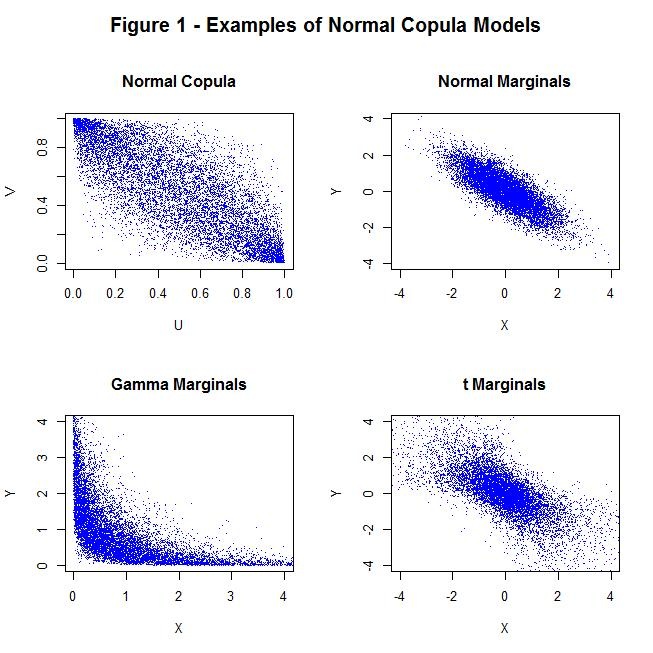
\includegraphics[width=0.9\textwidth]{copulas}
\end{figure}
univariate marginals leads to three different bivariate distributions.

	The forward implication of Sklar’s theorem means that every distribution can be rewritten in terms of a copula and univariate marginals. This suggests that copulas encode the dependency structure stripped from all the univariate marginal information like scale, shape and location. If a copula can be obtained, then the corresponding association structure can be studied via a copula density function. The importance of the forward implication can also be seen in \emph{Figure 1}, where three obviously different bivariate distributions, which are similar only with respect to a general negative association between random variables $X$ and $Y$, turn out to have identical association structure.
    
	From the Sklar’s theorem a couple useful corollaries follow that shed more light on how copulas are useful in constructing new multivariate distribution \citep{Joe1997,Nel2007}. The first corollary is an alternative representation of a multivariate probability density function: 
\newtheorem{cors}{Corollary}
\begin{cors}
For a differentiable p--dimensional distribution function with continuous quantile functions $F_1^{-1}, F_2^{-2}, \dots, F_p^{-1}$, the probability density function
\begin{align*}
f(x_1,x_2, \dots, x_p) = & \frac{\partial^p F(x_1, x_2, \dots, x_p)}{\partial x_1 \partial x_2 \cdots \partial x_p} = \\ 
& \frac{\partial^p C(F_1(x_1), F_2(x_2), \dots, F_p(x_p))}{\partial x_1 \partial x_2 \cdots \partial x_p} = \nonumber \\
& c(u_1, u_2, \dots, u_p)\prod_{i = 1}^p f(x_i)
\end{align*}
\end{cors} 
The usefulness of corollary 1 is that it provides an alternative way to construct a model by going directly to the probability density function.

	 Results presented so far provide an equation for construction of new models. However, any construction has to be preceded by finding useful copulas \citep{Joe1997,Nel2007}. The second corollary shows a simple way of obtaining a new copula:
\begin{cors}
Let $F$ be a p-dimensional distribution function with continuous quantile functions $F_1^{-1}, F_2^{-1}, \dots, F_p^{-1}$, then for every $(u_1, u_2, \dots u_p) \in [0, 1]^p$ 
\begin{equation*}
C(u_1, u_2, \dots u_p) = F(F_1^{-1}(u_1), F_2^{-1}(u_2), \dots, F_p^{-1}(u_p))
\end{equation*}
\end{cors}
The corollary 2 implies that if one can specify an existing multivariate distribution and derive its quantile functions, then its copula is easily recoverable using this equation. As a caveat, this method works only if quantile functions can be obtained, which is often difficult. There are other methods for finding new copulas, and the history of applying them produced a rich body of copulas to choose from \citep{Joe1997,Nel2007}. 

	In conclusion, taking the Sklar’s theorem and the two corollaries as a given, the problem of generalizing the Ratcliff diffusion model to have an association structure is clear. One must pick a copula and univariate marginal distributions for each processing component \citep{JohKot1994,JohKot1995}. Combining them using Sklar’s representation equation completes the construction. Thus, the methodology of copulas provides a solution to the main problem of the proposal.

%%%%%%%%%%%%%%%%%%%%%%%%%%%%%%%%%%%%%%%%%%%%%%%%%%%%%%%%%%%%%%%
\subsection{Predictive properties via Monte Carlo method}
	Once a multivariate distribution with an association structure is specified a new cognitive process model can be proposed. The remaining problems are to explore the model’s predictive properties, estimation properties and evaluating the model against real performance data. I will use statistical methods to solve all three problems. 
	
    First, obtaining predictions from a generalized diffusion model of simple decision making, under specified parameter values, requires solving a triple integral of the mixture model \citep{Tue2004}. The mixture density arises from integrating the Wiener first passage density with respect to a mixing density, which encodes associations between processing components via a copula. The complexity of the equation makes the triple integral analytically intractable, so the exact predictions cannot be obtained. Approximate predictions, however, can be calculated using the Monte Carlo method \citep{RobCas2004,GamLop2006}. The application of the Monte Carlo method amounts to setting up an integration problem as an expected value of a function of a variable calculated relative to some distribution. Using a data sample simulated from a distribution of interest and an appropriate law of large numbers, an expected value can be estimated using the arithmetic average of the function evaluated at each sampled draw.
	
    The mixture model of performance data fits with the Monte Carlo method since it can be interpreted as an expected value of the Wiener first passage density relative to a mixing density. Applying the method to obtain approximate predictions requires solving three problems: sampling from a copula, transforming each dimension according to a marginal quantile function and sampling from the Wiener first passage density. The first two problems can be solved with the open-source R programming environment that provides the package “Copula” to sample from a wide range of copulas and the R base package that contains routines for marginal quantile functions \citep{Rte2012,HofKoj2013}. I have a custom-made sampler for the Wiener FPD based on the random walk approximation \citep{TueMar2001}. All three pieces of software can be conveniently and flexibly combined in an R program to obtain approximate predictions for the proposed models.

%%%%%%%%%%%%%%%%%%%%%%%%%%%%%%%%%%%%%%%%%%%%%%%%%%%%%%%%%%%%%%%%%
\subsection{Bayesian inference via hierarchical models}
	The problems of testing proposed models against real performance data and establishing their estimation properties are methodologically tied. Bayesian statistical theory provides a powerful and general framework for solving both problems \citep{Ber1997,GelCar2013}. Recent technological developments made the Bayesian approach ripe for scientific use, and it is becoming popular in psychology, too \citep{EdwLin1963,MyuPit1997,MyuKar2008,PerVan2002,RouLu2005,RouLu22005,CraPer2010,VanTue2011}. The reasons for its appeal include representation of uncertainty with probability, coherent manipulation of uncertainty using probability calculus and ability to handle realistic models. I will adopt the Bayesian framework to solve the derivative problems of model estimation and evaluation.
	
    Unlike the frequentist framework, in the Bayesian framework model parameters are treated as random variables along with data. The full probability model, also called the Bayesian model, is at the center of analysis \citep{GelCar2013}. It requires specifying both the probability density of data and parameters. These two building blocks are assumed to be conditionally dependent in a way that the full joint density can be factored into a probability density of data given parameters, called the likelihood, and the probability density of parameters, called the prior. Given a data vector $\boldsymbol{X} \in \mathbb{R}^p$ and its parameter vector $\boldsymbol{\theta} \in \Theta \subseteq \mathbb{R}^m$, a Bayesian model
\begin{equation}
f(\boldsymbol{x}, \boldsymbol{\theta}) = f(\boldsymbol{x} \mid \boldsymbol{\theta})f(\boldsymbol{\theta})
\end{equation}
where $f(\boldsymbol{x} \mid \boldsymbol{\theta})$ is the likelihood function and $f(\boldsymbol{\theta})$ is the prior. The factorization property is useful for constructing new Bayesian models because it allows breaking the problem into manageable pieces, often consisting of common univariate distributions \citep{JohKot1994,JohKot1995}. 

	I will fit and test generalized cognitive process models by incorporating them into hierarchical Bayesian models \citep{Ber1997,GelCar2013}. This choice is motivated by the structure of performance data. A typical experiment generates multiple observations for each of several participants engaged in the same task \citep{RatMck2008,Wag2009}. When specifying a statistical model, the choice is often to either treat individual observations as coming from different sources or the same source \citep{RouLu2005,RouLu22005,RouMor2014}. Not pooling the data presupposes no relation between the individuals while completely pooling data ignores individual differences. However, for human performance data, it is more accurate to assume a middle ground. Real data varies among participants, but due to similarity in cognitive abilities and experimental treatment, participants share regularities. A hierarchical statistical model acknowledges this mixed structure by assuming that individual parameters are a random sample from a population, and introduces semi-pooling by fitting all the data simultaneously.
    
	In a hierarchical model, the parameter space can be factored out into parameters representing the individuals, and hyperparameters representing a population from which the individuals are sampled. With data $\boldsymbol{X} \in \mathbb{R}^p$ conditionally dependent on parameters $\boldsymbol{\theta} \in \Theta \subseteq \mathbb{R}^m$, and parameters conditionally dependent on hyperparameters $\boldsymbol{\psi} \in \Psi \subseteq \mathbb{R}^n$, a hierarchical model
\begin{equation}
f(\boldsymbol{x}, \boldsymbol{\theta}, \boldsymbol{\psi}) =
f(\boldsymbol{x} \mid \boldsymbol{\theta})
f(\boldsymbol{\theta} \mid \boldsymbol{\psi})
f(\boldsymbol{\psi})
\end{equation}
can be factored into the likelihood $f(\boldsymbol{x} \mid \boldsymbol{\theta})$, density of parameters $f(\boldsymbol{\theta} \mid \boldsymbol{\psi})$ and density of hyperparameters $f(\boldsymbol{\psi})$. Construction of a new Bayesian model amounts to selecting distributions for these three building blocks. I will construct hierarchical models to study estimation properties of generalized diffusion models and test them against benchmark data.

%%%%%%%%%%%%%%%%%%%%%%%%%%%%%%%%%%%%%%%%%%%%%%%%%%%%%%%%%%%%%%%%
\subsection{Blocked DE-MCMC sampler}
	Once a Bayesian model has been specified inference about unknown parameters can proceed by applying calculus of probabilities. In the Bayesian framework, parameter estimation is formalized as an instance of Bayes theorem 
\begin{equation}
\pi(\boldsymbol{\theta} \mid \boldsymbol{x}) = 
\frac{f(\boldsymbol{x} \mid \boldsymbol{\theta}) \pi(\boldsymbol{\theta})}
{\idotsint\limits_\Theta f(\boldsymbol{x} \mid \boldsymbol{\theta}) \pi(\boldsymbol{\theta})d\boldsymbol{\theta}},
\end{equation}
where $f(\boldsymbol{x} \mid \boldsymbol{\theta})$ is the likelihood function, $\pi(\boldsymbol{\theta})$ is the prior distribution and $\pi(\boldsymbol{\theta} \mid \boldsymbol{x})$ is the posterior distribution \citep{Ber1997,CasBer2002,GelCar2013}. The Bayes theorem implies that the posterior distribution is a compromise between the likelihood and the prior. Once the posterior is obtained various statistical inferences, such as point estimates, interval estimates, hypothesis tests and model checks, can be calculated.

	In practice, application of the Bayes theorem is complicated by the integral in the denominator. For instance, the first passage time density of the two-boundary Wiener process is intractable, so the posterior density cannot be calculated exactly. An approximation can be obtained by applying a special class of Monte Carlo algorithms that use Markov chains (MCMC) to sample from the posterior density \citep{RobCas2004,GamLop2006,GivHoe2012,GelCar2013}. The inference calculations can be rewritten as expected value problems, so a sample from the posterior density can be used to obtain approximate answers, including the complicated models like the hierarchical diffusion model \citep{PerVan2002,CraPer2010,VanTue2011}. 
    
	The aim of MCMC methods is to find regions of high probability density and explore them starting from an arbitrary starting point. Such stochastic search and exploration is conducted by simulating a discrete time, continuous state-space Markov chain \citep{KarTay1975,KarTay1981,Ros2014}. The mathematical description of the exploration is a transition kernel of a Markov chain, which is a conditional distribution function describing where the chain is likely to be next given where it is right now. MCMC samplers define a special kind of transition kernel that has a limiting distribution and is time-reversible. The sampler is constructed in such a way that the target distribution, from which a sample is sought, is equivalent to the limiting distribution. Thus, MCMC algorithms provide a method for sampling from arbitrary distributions for which a likelihood function can be specified. 
    
	I will use blocked differential evolution MCMC (DE-MCMC) to simulate from the posterior density \citep{Ter2006,TurSed2013}. The DE-MCMC is a genetic algorithm that uses a system of interrelated, multivariate Markov chains to explore the parameter space. One way to understand how an MCMC algorithm works is by examining its transition kernel, which consists of a proposal density that can explore the whole target space, and an acceptance probability function that enables visiting both high and low probability density regions.
    
	Once the chains are initialized, the DE-MCMC algorithm updates one chain at a time in a deterministic order. The proposal density perturbs the current position $\boldsymbol{\theta}_{k, i - 1}$ of the kth chain by adding independent noise $\varepsilon$ and a weighted difference of states of two other randomly picked chains $\upsilon(\boldsymbol{\theta}_{m, i - 1} - \boldsymbol{\theta}_{n, i - 1})$. The independent noise $\varepsilon$ is a proposal mechanism akin to many other samplers, such as Metropolis-Hastings, and requires tuning \citep{RobCas2004,GamLop2006}. The novel piece is using distances between states of other chains, weighted by a positive scalar, to update the current chain. The weight $\upsilon$ is the second tuning parameter. 
    
	The difference vectors reflect the geometry of the high probability regions, where most chains will reside if the algorithm is 

\vspace{5mm}
    
\centerline{\textbf{Figure 2 - Global DE-MCMC}}

\fbox{
\parbox{\textwidth}{
\begin{enumerate}
\item $\forall k \in \{1, 2, \dots, K\}$, initialize $\boldsymbol{\theta}_{k, 1} \ni \pi(\boldsymbol{\theta}_{k, 1} \mid \boldsymbol{x}) > 0$
\item for $i^{th}$ iteration in $2, 3, \dots, I$
\item \quad for $k^{th}$ chain in $1, 2, \dots, K$
\item \qquad Sample $\boldsymbol{\theta}_{m, i-1}, \boldsymbol{\theta}_{n, i-1}$ without replacement from \\ 
$\{\boldsymbol{\theta}_{1, i-1}, \boldsymbol{\theta}_{2, i-1}, \dots, \boldsymbol{\theta}_{K, i-1}\} \backslash \{\boldsymbol{\theta}_{k, i-1}\}$
\item \qquad Sample $\upsilon \sim \mathcal{U}(0.5, 1)$
\item \qquad Sample $\varepsilon \sim \mathcal{U}(-0.001, 0.001)$
\item \qquad Propose $\boldsymbol{\theta}^* = \boldsymbol{\theta}_{k, i-1} + \upsilon(\boldsymbol{\theta}_{m, i - 1} - \boldsymbol{\theta}_{n, i - 1}) + \varepsilon$
\item \qquad Sample $\alpha \sim \mathcal{U}(0, 1)$
\item \qquad if $\alpha < \frac{\pi(\boldsymbol{\theta}^* \mid \boldsymbol{x})}{\pi(\boldsymbol{\theta}_{k, i-1} \mid \boldsymbol{x})}$, then $\boldsymbol{\theta}_{k, i} = \boldsymbol{\theta}^*$
\item \qquad else $\boldsymbol{\theta}_{k, i} = \boldsymbol{\theta}_{k, i-1}$
\item \quad end for
\item end for
\end{enumerate}
	}
}

\vspace{5mm}

\noindent working, and improve sampling. Given the proposed value $\boldsymbol{\theta}^*$, the acceptance probability function determines whether the chain moves or stays. The DE-MCMC uses the same kind of acceptance function as Metropolis-Hastings. Figure 2 gives an algorithmic representation of such a transition kernel. The steps describe a global DE-MCMC algorithm that moves chains through the whole parameter space at once.

	The reason for choosing blocked DE-MCMC is because it works well with highly correlated parameter spaces \citep{TurSed2013}. Correlated parameter space holds true for the Ratcliff diffusion model \citep{RatTue2002}, and is likely to be inherited by the generalized models. In addition, real data problems, including applying generalized diffusion models to reaction times and accuracy, involve high-dimensional parameter spaces. Without partitioning the parameter space into blocks the computational efficiency of the algorithm is seriously reduced. 
    
    A common partitioning scheme, called Gibbs sampling, breaks apart the parameter space into univariate blocks \citep{RobCas2004,GamLop2006,GelCar2013}. However, due to correlations between parameters in cognitive process models, it will be more efficient to work with blocks of several correlated dimensions. Exploring the space in several dimensions simultaneously will increase chances of proposing an acceptable move. Hence, the best, if not always obvious, blocking scheme is to group correlated parameters together and keep relatively independent parameters separate. Figure $3$ shows an example of a blocked DE-MCMC for a hierarchical model of $J$ participants each generating $N$ normal observations 
\begin{gather}
\psi_{\mu} \sim \mathcal{N}(0, 10000), \quad 
\chi_{\mu} \sim \mathcal{G}(0.01,0.01) \nonumber \\
\psi_{\sigma^2} \sim \mathcal{G}(0.01, 0.01), 
\quad \chi_{\sigma^2} \sim \mathcal{G}(0.01,0.01) \nonumber \\
\mu_j \sim \mathcal{N}(\psi_{\mu}, \chi_{\mu}), 
\quad \sigma_j^2 \sim \mathcal{TN}(\psi_{\sigma^2}, \chi_{\sigma^2}) \nonumber \\
X_{n, j} \sim \mathcal{N}(\mu_j, \sigma_j^2) \nonumber
\end{gather}
In this example, the blocked DE-MCMC explores the model’s parameter space by updating one pair of means and variances at a time.

	As any other MCMC algorithm, the DE-MCMC will generate a sample from the posterior that is autocorrelated and is only guaranteed to converge to the target distribution asymptotically \citep{RobCas2004,GamLop2006}. To ensure the quality of samples, before calculating any inferences, I will use graphical and numerical methods to diagnose convergence of chains to the target density. These methods are heuristics that do not guarantee convergence, but their failure guarantees failure of convergence.
    
    The standard graphical tools will include trace plots to examine the time series of samples, and autocorrelation plots to gauge mixing of the sampler, or how well the chains move around. I will use the trace plot by overlaying many chains and observing if they stabilize around the same point, which is strong evidence for convergence. Also, the trace plot will help to determine the burn-in period, the initial iterations that take the algorithm to find the high density region from an initial state. In contrast, the autocorrelation plot will assist in checking the proposal tuning, and whether the blocking scheme combines highly correlated parameters. High autocorrelation would indicate issues with either/both of these design choices.

\vspace{5mm}

\centerline{\textbf{Figure 3 - Blocked DE-MCMC}}
\fbox{
\parbox{\textwidth}{
\begin{enumerate}
\item $\forall k \in \{1, 2, \dots, K\}$, initialize $\boldsymbol{\theta}_{k, 1} \ni \pi(\boldsymbol{\theta}_{k, 1} \mid \boldsymbol{x}) > 0$
\item for $i^{th}$ iteration in $2, \dots, I$
\item \quad for $k^{th}$ chain in $1, \dots, K$ use the DE-MCMC kernel to sample
\item \qquad $(\psi_{\mu}, \chi_{\mu})^i \mid (\mu_1, \sigma_1^2, \mu_2, \sigma_2^2, \dots, \mu_J, \sigma_J^2)^{i-1}$
\item \qquad $(\psi_{\sigma^2}, \chi_{\sigma^2})^i \mid (\mu_1, \sigma_1^2, \mu_2, \sigma_2^2, \dots, \mu_J, \sigma_J^2)^{i-1}$
\item \qquad for $j^{th}$ participant in $1, 2, \dots, J sample$
\item \quad \qquad$ (\mu_j, \sigma_j^2) \mid (\psi_{\mu}, \chi_{\mu}, \psi_{\sigma^2}, \chi_{\sigma^2})^{i-1}$
\item \qquad end for
\item \quad end for
\item end for
\end{enumerate}
	}
}

\vspace{5mm}
	
    Numerically, I will calculate the \citet{GelRub1992} convergence statistic, the potential reduction scale factor (PRSF), that detects stationarity of chains by comparing between-chain to within-chain variance \citep{BroGel1998}. For $i = 1, 2, \dots, m$ chains, let $\theta_{i, j}$  be $j^{th}$ of $n$ iterations of a univariate parameter $\theta$ with mean $\mu$ and variance $\sigma^2$, then the between-chain variance
    
\begin{equation}
B = \frac{n}{m(n-1)}\sum_{i=1}^m(\theta_i - \overline\theta)^2
\end{equation}
and the within-chain variance

\begin{equation}
W = \frac{1}{m(n-1)}\sum_{i=1}^m \sum_{j=1}^n(\theta_{i,j} - \overline\theta_j)^2 = \frac{1}{m}\sum_{i=1}^m s_i^2
\end{equation}
are combined to calculate the pooled posterior variance estimate 

\begin{equation}
\hat V = \frac{n}{n-1}W + (\frac{1}{mn} + \frac{1}{n})B
\end{equation}
Then a corrected PRSF

\begin{equation}
\hat R = (\frac{d+3}{d+1})\frac{\hat V}{W}
\end{equation}
with the degrees of freedom

\begin{equation}
d \approx \frac{2 \hat V^2}
{\operatorname{\hat {var}} (\hat V)}
\end{equation}
and the variance estimate

\begin{eqnarray}
\operatorname{\hat {var}}(\hat V) & = & (\frac{n-1}{n})^2 \frac{1}{m} \operatorname{\hat {var}}(s_j^2) + \frac{m+1}{mn}^2 \frac{2}{m-1}B^2 + \nonumber \\
& + & 2\frac{(m+1)(n-1)}{m^2n}(\operatorname{\hat {cov}}(s_j^2,\overline\theta_j) - 2\overline\theta\operatorname{\hat {cov}}(s_j^2,\overline\theta))
\end{eqnarray}
I will treat a posterior sample with $1 \leq \hat R \leq 1.05$.

%%%%%%%%%%%%%%%%%%%%%%%%%%%%%%%%%%%%%%%%%%%%%%%%%%%%%%%%%%%%%%%%
\subsection{Model selection via Bayesian predictive information criterion}
	Model selection, a kind of statistical inference, arises when several competing models are proposed to describe the same data. The criteria of selection can be broken down into qualitative and quantitative kinds \citep{MyuKar2008,ShiLee2008,VanMat2014}. In psychology, interpretability of the parameters and plausibility of explanation it provides for data are important qualitative criteria. The generalized diffusion models I intend to propose will inherit the simple decision making interpretation for non-association parameters, and the association parameters may be interpreted as processing coordination imposed by cognitive control processes. The explanatory plausibility cannot be judged a priori, and will be determined by applying the models to real performance data.
    
	In contrast to qualitative considerations, a common quantitative approach to model selection is based on model generalizability \citep{GelHwa2013}. Generalizability is defined as model’s predictive accuracy for out-of-sample data collected under the same conditions. A model with better generalizability indicates a better approximation of the underlying regularity. One way to interpret this from the Bayesian perspective is to consider the posterior predictive distribution 
\begin{equation}
f(\boldsymbol{y} \mid \boldsymbol{x}) = \int\limits_{\Theta} f(\boldsymbol{y} \mid \theta)\pi(\boldsymbol{\theta} \mid \boldsymbol{x})d\boldsymbol{\theta} = \operatorname{E_{\boldsymbol{\theta} \mid \boldsymbol{x}}}[f(\boldsymbol{y} \mid \boldsymbol{\theta}],
\end{equation}
where $\boldsymbol{y} \in \mathcal{R}^p$ is future data, $\boldsymbol{x} \in \mathcal{R}^p$ is observed data and $\boldsymbol{\theta} \in \Theta^n \subseteq \mathcal{R}^m$ is parameter vector. The posterior predictive distribution encodes all the predictions of an updated Bayesian model. A generalizability criterion should support selection of a model with the most accurate posterior predictive distribution.

	The various proposals for how to calculate out-of-sample predictive accuracy can be decomposed into two parts: an estimate of predictive accuracy based on observed data and a penalty term. The penalty term is a correction for overfitting due to use of the same data both for parameter estimation and model evaluation. The overfitting of a model to data is driven by model complexity, so the penalty term quantifies model complexity. A popular and easy-to-calculate generalizability measure is deviance information criterion (DIC) \citep{SpiBes2002}, which decomposes additively into the measure of fit

\begin{equation}
\overline D = \operatorname{E_{\boldsymbol{\theta} \mid \boldsymbol{x}}}[-2\operatorname{log}f(\boldsymbol{x} \mid \boldsymbol{\theta})]
\end{equation}
and the penalty term

\begin{equation}
p_D = \operatorname{E_{\boldsymbol{\theta} \mid \boldsymbol{x}}}[-2\operatorname{log}f(\boldsymbol{x} \mid \boldsymbol{\theta})] + 2\operatorname{log}f(\boldsymbol{x} \mid \operatorname{E_{\boldsymbol{\theta} \mid \boldsymbol{x}}}[\boldsymbol{\theta}] + c
\end{equation}
It was developed to work with hierarchical Bayesian models where complexity is quantified with effective number of parameters $p_D$. The issue with DIC is that it tends to pick overfitted models \citep{GelHwa2013}. 

	Bayesian predictive information criterion, 

\begin{equation}
BPIC = \overline D + 2p_D
\end{equation}
was developed by \citet{Ano2007,Ano2011}, to correct bias in DIC, which turns out to be equivalent to doubling the penalty term. For a posterior sample obtained by an MCMC algorithm, BPIC can be easily estimated with 

\begin{equation}
\hat{BPIC} = -\frac{6}{N}\sum_{i=1}^N \operatorname{log}f(\boldsymbol{x} \mid \boldsymbol{\theta_i}) + 4\operatorname{log}f(\boldsymbol{x} \mid  \boldsymbol{\overline\theta})
\end{equation}
 
	There are two conditions under which BPIC is applicable to hierarchical Bayesian models \citep{Ano2011}. First, the derivation assumes that the likelihood model does not include the exact generating distribution, but is not far from the true model. The second condition is marginal posterior distributions are unimodal and not too skewed. The empirical success of the Ratcliff diffusion model \citep{RatMck2008,Wag2009,VanTue2011} and prior hierarchical fits of the model suggest that both of these conditions hold. Therefore, I will use BPIC for model selection when fitting proposed models to benchmark data. 

%%%%%%%%%%%%%%%%%%%%%%%%%%%%%%%%%%%%%%%%%%%%%%%%%%%%%%%%%%%%%
\subsection{Model checking using posterior predictive checks}
	Model selection based on predictive accuracy is useful for ordering a set of competing models and selecting the one that will make the best predictions for future observations generated by the same process. The output is a best model relative to the competitors. However, because selection criteria are scalar quantities, they do not reveal which features of data the best model predicts well and which feature it misses. That is, it does not give a sense of absolute fit of a model to data. It is possible that a model may be best in a set of alternatives, but miss all the important features of data. Thus, in addition to model selection, it is important to directly check a model against data. A Bayesian approach to check the absolute fit and misfit of a model is to compare its posterior predictive distribution to observations. 

	The comparison between observations and posterior predictive distribution is formalized in the method of posterior predictive checks \citep{GelGoe2000,GelCar2013}. I will concentrate on the graphical method rather than numerical. The procedure requires selecting a pivotal, discrepancy statistic $S(\:)$ that captures some interesting data feature. For example, one may consider the quantile set $\{0.1, 0.3, 0.5, 0.7, 0.9\}$ for both correct and error response times as important features that a model should capture. Then, a discrepancy statistic $S(\boldsymbol{x}_{obs})$ is calculated for the observed data. The model’s predictions for the statistic have to reflect uncertainty in the parameter, so a sample, say 250, is taken randomly from the estimated posterior. For each parameter value a data set is generated of the same size as the observed data, and the discrepancy statistics $S(\boldsymbol{y}_{rep,1}), S(\boldsymbol{y}_{rep,2}), \dots, S(\boldsymbol{y}_{rep,250})$  are calculated. Then, one can plot the $S(\boldsymbol{x}_{obs})$ against the posterior predicted distribution of the statistic. The location of the observed value relative to the high density region will reveal consistency between the model and observations. 
    
	For performance data one could overlay the observed versus predicted quantile-probability function to determine how well the proposed models of simple decision making capture the joint behavior of reaction times and responses. I will use the posterior predictive checks to test adequacy of proposed models with respect to central features of benchmark data.


%%%%%%%%%%%%%%%%%%%%%%%%%%%%%%%%%%%%%%%%%%%%%%%%%%%%%%%%%%%%%%%
\section{Proposed models}
\subsection{Models of across-trial variability}
	The main problem addressed by this thesis is development of cognitive process models capable of recovering an association structure between processing components from response times and response proportion data. I propose two new diffusion models that could in principle solve this problem. 

	Both models take the Wiener process as a description of the decision process involved in simple decision making, but they differ in the mixing densities that describe across-trial variability. I will work with bias parameterization, and the starting point can always be recovered from posterior samples of bias. The mixing densities describe variation and covariation in the processing components including drift rate, bias and non-decision time. Construction of a new mixing density amounts to specifying a new multivariate density. Using Sklar’s theorem the problem of constructing a new multivariate density can be broken down to selecting a copula and marginal probability density functions.
    
	In proposing the two mixing densities I aimed to choose both flexible copulas and marginals. First, the copulas have to be flexible to encode different types of association structures. Within the set of existing copulas, many copulas, regardless of the dimension, are governed by a single parameter that induces a particular kind of association \citep{Joe1997,Nel2007}. For example, Archimedean copulas are controlled by a single parameter and encode the same lower tail, or upper tail, or all-positive associations for all pairs of variables. However, since there is no prior information available about the association structure between processing components underlying simple decision making, it is sensible to start modeling with more flexible copulas. I interpret flexibility as being able to have different associations for each pair ranging from full negative to full positive dependence. 
    
	The elliptical class of copulas satisfies the flexibility criterion. Specifically, I propose using the normal and t copulas from the elliptical class to encode association structure into the model of simple decision making. The first proposed model has a normal copula 

\begin{eqnarray}
C_1 (\boldsymbol{u} \mid \rho_{1,2},\rho_{1,3},\rho_{2,3}) = \Phi_3(\Phi^{-1}(u_1),\Phi^{-1}(u_2),\Phi^{-1}(u_3) \mid \boldsymbol{P}_1) = \nonumber \\ \int_{-\infty}^{\Phi^{-1}(u_1)}\int_{-\infty}^{\Phi^{-1}(u_2)}\int_{-\infty}^{\Phi^{-1}(u_3)}\operatorname{det}(2\pi\boldsymbol{P}_1)^{-\frac{1}{2}}\operatorname{exp}(-\frac{1}{2}\boldsymbol{x}^T\boldsymbol{P}_1\boldsymbol{x})d\boldsymbol{x}
\end{eqnarray}
where $\Phi_3(\:)$ is a three dimensional standard normal distribution function and $\Phi^{-1}(\:)$ is the normal quantile function. Note that it is derived using corollary 2. The copula is governed by association parameters $\rho_{i,j} \in [-1, 1]$ for $i, j = 1, 2, 3$ through a positive definite association matrix

\begin{equation}
\boldsymbol{P}_1 = \left[ \begin{array}{ccc}
1 & \rho_{1, 2} & \rho_{1, 3} \\
\rho_{1, 2} & 1 & \rho_{2, 3} \\
\rho_{1, 3} & \rho_{2, 3} & 1
\end{array}
\right].
\end{equation}
From Sklar’s theorem, coupling the normal copula with the normal marginals will result in the multivariate normal CDF, but substituting some other marginals into the normal copula will result in novel probability distributions. 

	Similarly, the second proposed model will have a t copula 
    
\begin{eqnarray}
C_2(\boldsymbol{u} \mid \rho_{1,2},\rho_{1,3},\rho_{2,3},\omega) = T_3(t^{-1}(u_1 \mid \omega),t^{-1}(u_2 \mid \omega),t^{-1}(u_3 \mid \omega) \mid \boldsymbol{P}_2) = \nonumber \\ 
\int_{-\infty}^{t^{-1}(u_1 \mid \omega)}\int_{-\infty}^{t^{-1}(u_2 \mid \omega)}\int_{-\infty}^{t^{-1}(u_3 \mid \omega)}\frac{\Gamma(\frac{\omega+d}{2})}{\Gamma(\frac{\omega}{2})\sqrt{(\omega\pi)^d \operatorname{det}(\boldsymbol{P}_2)}}\left(1+\frac{\boldsymbol{x}^T\boldsymbol{P}_2^{-\frac{1}{2}}\boldsymbol{x}}{\omega}\right),
\end{eqnarray}
where $T_3$ is a three dimensional t cumulative distribution function, $\Gamma(\:)$ is a univariate gamma function and $t^{-1}(\:)$ is a t quantile function. t copula is also derived via corollary 2. The t copula is similarly parameterized with an association matrix  

\begin{equation}
\boldsymbol{P}_2 = \left[ \begin{array}{ccc}
1 & \rho_{1, 2} & \rho_{1, 3} \\
\rho_{1, 2} & 1 & \rho_{2, 3} \\
\rho_{1, 3} & \rho_{2, 3} & 1
\end{array}
\right],
\end{equation}
but also has a parameter $\omega > 0$ that influences heaviness of the tails. The parameter introduces an additional flexibility that controls probability of extreme values in the tails and variable combinations that contradict the association structure. For example, if association between two variables is positive, it is unlikely to observe a pair of values where one point has high magnitude and the second point has low magnitude. Presence of rare events is predicted for finite values of $\omega$, however as $\omega \to \infty$ the t copula converges to the normal copula. Thus, the cognitive process model based on the t copula is a further generalization of the normal copula that allows modeling associations between processing components that sometimes take unusual values, that is break the general coordination pattern.

	To complete the construction of the mixing densities, Sklar’s theorem dictates that one specifies the marginal distributions for each variable component of processing. The choice of marginal distributions is meant to preserve successful fit of the Ratcliff model, which is pretty robust to variation in distribution assumptions \citet{Rat2013}, but also includes distributions that can take more flexible shapes relative to a uniform variate. 
    
	For the drift rate $\delta$, in line with the Ratcliff model, I will assign a normal distribution. I will replace the continuous uniform assumption for the non-decision parameter $t^{er}$ with a truncated normal distribution, which adds more flexibility to the shape. The truncation on both the left and right side can be fixed using a list of $23$ studies fitting the Ratcliff diffusion model \citep{MatWag2009}. I will take the minimum and maximum values ($0.206$ and $0.942$) from the reported studies as truncation points, $a < b$.  Lastly, the bias parameter $\beta$ will follow a beta distribution because of its flexibility in shape. Overall, the univariate marginals are 

\begin{eqnarray}
\delta & \sim & \mathcal{N}(\nu, \eta) \nonumber \\
\beta & \sim & \mathcal{B}(\lambda, \gamma) \nonumber \\
t^{er} & \sim & \mathcal{TN}(\chi,\phi,a,b)
\end{eqnarray}
 
Applying Sklar’s theorem to the specified copulas and marginals will result in $i = 1, 2$ new mixing distributions of the form
\begin{equation}
F_i(\delta,\beta,t^{er}) = C_i(F_{\delta}(\delta),F_{\beta}(\beta),F_{t^{er}}(t^{er})),
\end{equation}
from which one can easily obtain mixing densities by a mixed derivative
\begin{equation}
\frac{\partial^3}{\partial\delta\partial\beta\partial t^{er}}F_i(\delta,\beta,t^{er}) = c_i(F_{\delta}(\delta),F_{\beta}(\beta),F_{t^{er}}(t^{er}))f_{\delta}(\delta),f_{\beta}(\beta),f_{t^{er}}(t^{er})
\end{equation}
 
	The copula density and marginal densities have analytic expressions that are readily available \citep{Nel2007,CasBer2002,JohKot1994,JohKot1995}. Direct application of the Sklar’s theorem ensures that both models of parameter variability are valid distributions. This completes construction the construction of two new models. 
    
	Testing the usefulness of proposed models will require combining the new mixing densities with the Wiener first passage density into mixture densities to predict how response times and responses are jointly distributed. This is the topic of the first proposed study.

%%%%%%%%%%%%%%%%%%%%%%%%%%%%%%%%%%%%%%%%%%%%%%%%%%%%%%%%%%%%%%%%
\section{Proposed studies}
\subsection{Study A – predictive properties}
\indent The first study will examine predictive properties of the proposed models. The predictive properties are a pattern of effects on the marginal and joint features of performance data attributable to an association structure. The data features I will examine are the probability density functions of the correct and error response times, the $\{0.025, 0.1, 0.3, 0.5, 0.7, 0.9, 0.975\}$ quantile set of the correct and error response times, and probabilities of response one and two. The combination of these features allows graphical and quantitative comparison of the two proposed diffusion models with association structure and the independent diffusion model.  

	To get a comprehensive understanding of how an association structure effects chosen data features I will examine a collection of parameter combinations that reflect estimates recovered in reported studies and several association structures \citep{MatWag2009}. The combinations of non-association parameters will resemble a typical experimental study where stimulus difficulty is manipulated on a trial basis, and speed/accuracy instructions and decision bias are manipulated on a block basis. The study will have four stimulus difficulty levels spanning near chance to near-ceiling performance, speed and accuracy emphases, and bias/no-bias conditions. Conditions affecting perceptual and response execution are assumed to be constant. Environmental factors affecting variability in decision process components are assumed to induce slower error response times relative to correct response times, faster error response times or symmetric response times. \emph{Table 1} contains non-association parameter values representing the proposed conditions based on ranges and means from 23 studies fitting the Ratcliff diffusion model \citep{MatWag2009}.
    
\begin{table}[H]
\centering
\caption{\textbf{Non-association parameters}}
\begin{tabular}{|l*{9}{|c}|r|}
\hline
Set & $\alpha$ & $\nu_1$ & $\nu_2$ & $\nu_3$ & $\nu_4$ & $\lambda$ & $\chi$ & $\eta$ & $\gamma$ & $\phi$ \\ \hline
1 & 0.10 & 0.00 & 0.10 & 0.20 & 0.40 & 0.50 & 0.250 & 0.12 & 0.05 & 0.05 \\ \hline
2 & 0.10 & 0.00 & 0.10 & 0.20 & 0.40 & 0.50 & 0.250 & 0.05 & 0.15 & 0.05 \\ \hline
3 & 0.10 & 0.00 & 0.10 & 0.20 & 0.40 & 0.50 & 0.250 & 0.01 & 0.01 & 0.05 \\ \hline
4 & 0.10 & -0.20 & -0.05 & 0.05 & 0.20 & 0.65 & 0.250 & 0.12 & 0.05 & 0.05 \\ \hline
5 & 0.10 & -0.20 & -0.05 & 0.05 & 0.20 & 0.65 & 0.250 & 0.05 & 0.15 & 0.05 \\ \hline
6 & 0.10 & -0.20 & -0.05 & 0.05 & 0.20 & 0.65 & 0.250 & 0.01 & 0.01 & 0.05 \\ \hline
7 & 0.20 & 0.00 & 0.05 & 0.10 & 0.20 & 0.50 & 0.250 & 0.12 & 0.05 & 0.05 \\ \hline
8 & 0.20 & 0.00 & 0.05 & 0.10 & 0.20 & 0.50 & 0.250 & 0.05 & 0.15 & 0.05 \\ \hline
9 & 0.20 & 0.00 & 0.05 & 0.10 & 0.20 & 0.50 & 0.250 & 0.01 & 0.01 & 0.05 \\ \hline
10 & 0.20 & -0.10 & -0.025 & 0.025 & 0.10 & 0.65 & 0.250 & 0.12 & 0.05 & 0.05 \\ \hline
11 & 0.20 & -0.10 & -0.025 & 0.025 & 0.10 & 0.65 & 0.250 & 0.05 & 0.15 & 0.05 \\ \hline
12 & 0.20 & -0.10 & -0.025 & 0.025 & 0.10 & 0.65 & 0.250 & 0.01 & 0.01 & 0.05 \\ \hline
\end{tabular}
\end{table}

    Under each of the experimental conditions, I will examine several association structures with low, medium and high levels of association between processing components. The association parameters for the normal and t copulas will be matched to ensure the same level of association. Kendall’s association coefficient, which measures the amount of monotonic association between two variables, suggests a way to match the two copulas. A convenient fact from copula theory is that Kendall’s coefficient depends only on a copula \citep{Joe1997,Nel2007}. For elliptical copulas used in the proposed models the Kendall’s coefficient is
\begin{equation}
\psi = \frac{2}{\pi}arcsin(\rho),
\end{equation} 
where $\rho$ is an association parameter of either normal or t copula. This expression implies that the proposed models with the same association parameters will have the same level of associations and differ only in the tail dependence. 

	\emph{Table 2} contains values for association parameters for several types of association structures. The structures reflect a few of many possible association
\begin{table}[H]
\centering
\caption{\textbf{Association parameters}}
\label{tab:2}
\begin{tabular}{|l|c|c|r|}
\hline
Set & $\rho_{\nu,\lambda}$ & $\rho_{\nu,\gamma}$ & $\rho_{\gamma,\lambda}$ \\ \hline
1 & 0.15 & 0.15 & 0.15 \\ \hline
2 & 0.50 & 0.50 & 0.50 \\ \hline
3 & 0.85 & 0.85 & 0.85 \\ \hline
4 & -0.15 & -0.15 & -0.15 \\ \hline
5 & -0.50 & -0.50 & -0.50 \\ \hline
6 & -0.85 & -0.85 & -0.85 \\ \hline
7 & -0.15 & -0.15 & 0.15 \\ \hline
8 & -0.50 & -0.50 & 0.50 \\ \hline
9 & -0.85 & -0.85 & 0.85 \\ \hline
\end{tabular}
\end{table}
\noindent patterns that could exist under typical experimental conditions. The all-positive and all-negative structures will allow establishing effects of association magnitude, sign and their interaction on the performance data. The mixed structure will also allow establishing effects of magnitude, but under mixed signs.  

	Some preliminary calculations suggest that introduction of a mixing density with dependent components will mostly affect the right tail of the mixture density. Specifically, the probability of extremely slow response times will decrease, and the thickness of the right tail will decrease, depending on the pattern and strength of associations. For instance, strong positive association among all processing component leads to decreases in the tail features for the correct response times and to increases for the error response times. The effects are manifest either in graphical representation of the correct and error probability densities, or the ${0.7, 0.9, 0.975}$ quantile set. The effects persist, but are not identical across several empirically consistent combinations of non-association parameters. This suggests that the proposed study exploring a rich set of parameter combinations should provide an adequate understanding of how addition of an association structure to the diffusion model effects predictions of the response time and response data. 

%%%%%%%%%%%%%%%%%%%%%%%%%%%%%%%%%%%%%%%%%%%%%%%%%%%%%%%%%%%%%%%%
\subsection{Study B – estimation properties}
	Study B will address the problem of parameter recovery of the proposed models using Bayesian inference. Accurate estimation of parameters is necessary to draw reliable inferences about cognition from data. Analytical examination of estimation properties of the proposed models is intractable, so I will use Monte Carlo simulation \citep{RobCas2004,GamLop2006,GelCar2013}. The overall constraints on how I specify dimensions of the study are related to applying the proposed models to the benchmark data in Study C \citep{RatRou1998}.

	The abstract structure of the benchmark dataset is equivalent to a few participants observed under a multifactorial design, with a moderate number of observations per cell. \emph{Table 3} contains proposed parameters that fall in the ranges of values that are recovered in real experiments \citep{MatWag2009}.
\begin{table}[H]
\centering
\caption{\textbf{True parameters}}
\label{tab:3}
\begin{tabular}{|l*{11}{|c}|r}
\hline
Subject & $\alpha$ & $\nu_1$ & $\nu_2$ & $\nu_3$ & $\nu_4$ & $\lambda$ & $\chi$ & $\eta$ & $\gamma$ & $\phi$ \\ \hline
I & 0.10 & -0.20 & -0.05 & 0.05 & 0.20 & 0.55 & 0.225 & 0.10 & 0.15 & 0.05 \\ \hline
I & 0.20 & -0.10 & -0.025 & 0.025 & 0.10 & 0.60 & 0.225 & 0.10 & 0.15 & 0.05 \\ \hline
II & 0.08 & -0.25 & -0.10 & 0.10 & 0.25 & 0.50 & 0.250 & 0.12 & 0.20 & 0.08 \\ \hline
II & 0.16 & -0.13 & -0.05 & 0.05 & 0.13 & 0.55 & 0.250 & 0.12 & 0.20 & 0.08 \\ \hline
III & 0.12 & -0.15 & -0.08 & 0.08 & 0.15 & 0.60 & 0.275 & 0.08 & 0.18 & 0.12 \\ \hline
III & 0.18 & -0.075 & -0.04 & 0.04 & 0.075 & 0.65 & 0.275 & 0.08 & 0.18 & 0.12 \\
\hline
\end{tabular}
\end{table}
\noindent I will assume a design with three participants undergoing trial-wise manipulation of stimulus quality, and block-wise manipulation of speed/accuracy instructions. For each participant, I will use association values specified in \emph{Table 2} (page \pageref{tab:2}) that span from low to high level of association. The degrees of freedom for the t copula will be 5 to ensure a scenario where extreme combinations of processing components are likely. For all the stimulus/instruction combinations I will sample 50, 150, and 500 observations since these values are common from developmental to cognitive psychology \citep{Luc1986,Wag2009,RouLu2005}.
    
	Sampling will be conducted under assumption of independent observations, thus ignoring the trend and autocorrelation present in real data \citep{PerVan2002,CraPer2010}. However, the experimental design somewhat alleviates the issue of sequential dependencies. Because stimulus is manipulated on each trial, the analysis is done on groups of trials pulled at different trial points, as opposed to the actually observed sequence. Such extraction breaks the temporal structure and amounts to a kind of thinning process (i.e. removing elements of a point stochastic process according to a predefined rule \citep{RobCas2004,GamLop2006,GelCar2013,Ros2014}. The dependencies are reduced with the greater number of stimulus quality conditions. The benchmark data has 66 stimulus quality/instruction conditions, so the independence assumption seems to be a plausible approximation that will generalize conclusions to fitting new diffusion models to the benchmark data.
    
	I propose three hierarchical Bayesian models whose estimation properties will be explored under the specified simulation conditions. Using the factorization property of Bayesian models I will specify the likelihood, priors and hyperpriors in order. For each participant, the data set will contain $n$ observations, equally split between $j = 1, 2, \dots, 4$ stimulus levels and $k = 1, 2$ instruction conditions. The $i^{th}$ observation of response time and response has a two-boundary Wiener first passage time probability density
\begin{equation}
f(t_{i,j,k}^{rt}, r_{i,j,k} \mid \alpha_k, \delta_{i,j,k}, \beta_{i,j,k}, \tau_{i,j,k}^{er}),
\end{equation}
where processing parameters reflect assumption of effect of instructions on the threshold, and across-trial variability. I will assume that each observation is independent conditional on the processing parameters. 

	The second building block is the prior. The proposed mixing densities act as priors in the Bayesian diffusion model. Processing parameters undergo fluctuations from trial to trial according to a copula-based density
\begin{eqnarray}
f(\delta_{i,j,k},\beta_{i,j,k},\tau_{i,j,k}^{er} \mid \nu_{i,j},\eta,\lambda_k,\gamma_k,\chi,\phi,\rho_{\tau^{er},\delta},\rho_{\beta,\delta},\rho_{\tau^{er},\beta}) = \nonumber \\
c(F_{\delta}(\delta_{i,j,k}),F_{\beta}(\beta_{i,j,k}),F_{t^{er}}(\tau_{i,j,k}^{er}) \mid \rho_{\tau^{er}.\delta}, \rho_{\beta,\delta},\rho_{\tau^{er},\beta}) \times \nonumber \\
f_{\delta}(\delta_{i,j,k} \mid \nu_{i,j}, \eta)f_{\beta}(\beta_{i,j,k} \mid \lambda_k,\gamma_k)f_{\tau^{er}}(\tau_{i,j,k}^{er} \mid \chi, \phi, 0.1, \operatorname{min}(\tau^{er})),
\end{eqnarray}
where $c(\:)$ defines a density for a copula, either an independent, a normal or a t, and incorporates three different association structures. The remaining marginal densities are normal, beta, truncated normal, respectively, and are assumed to be the same for all the models. Finally, the prior specification is complete by assuming the threshold parameter
\begin{equation}
\alpha_k \sim \mathcal{U}(0.01, 0.45).
\end{equation}

	Treating the association model as a prior fits neatly with the Bayesian computation, where MCMC can be used to approximate the posterior distribution and naturally implements the difficult integral required to specify the mixture model of performance data. Marginalizing over the trial specific parameters is simply dropping nuisance parameters from analysis.
    
	The last building block is the hyperprior density. I will use informed priors based on long experience with the Ratcliff diffusion model \citep{MatWag2009} for the non-association parameters, but association parameters will be assigned diffuse priors to express ignorance about this type of parameter. The full hyperprior density will differ for each model reflecting their association structure. The independent copula diffusion model is assigned the following hyperpriors
\begin{gather}
\nu_{i,j} \sim \mathcal{U}(-1.00, 1.00) \nonumber \\
\eta \sim \mathcal{U}(0, 0.3) \nonumber \\
\lambda_k \sim \Gamma(2, 3), \quad \gamma_k \sim \Gamma(2, 3) \nonumber \\
\chi \sim \mathcal{U}(0.10, 1.00), \quad \phi \sim \mathcal{U}(0, 0.35)
\end{gather}

The normal copula diffusion model adds the association parameters hyperpriors
\begin{eqnarray}
\rho_{\tau^{er},\delta} \sim \mathcal{U}(-1.00, 1.00) \nonumber \\
\rho_{\beta,\delta} \sim \mathcal{U}(-1.00, 1.00) \nonumber \\
\rho_{\tau^{er},\beta} \sim \mathcal{U}(-1.00, 1.00)
\end{eqnarray}

Finally, the t copula diffusion model adds the degrees of freedom hyperprior
\begin{equation}
\omega \sim \Gamma(1, 1)
\end{equation}
 
	To establish statistical properties of the proposed Bayesian models, each parameter-by-sample size combination will be simulated 200 times to obtain a sampling distribution of posterior means of all the unknown parameters, for the three proposed models. I will use root mean squared error
\begin{equation}
RMSE = \sqrt{\frac{1}{m}\sum_{i=1}^M (\theta^{true} - \operatorname{\hat E}_{\theta \mid x}[\theta]_i)^2}
\end{equation}
as a loss function to measure quality of hierarchical estimates because it combines both bias and variability of an estimator \citep{CasBer2002,RatTue2002,RouLu2005}. Successful application of the proposed models will rely on obtaining accurate estimates with small sample sizes and showing consistency of estimation as the sample size grows. Both of these requirements can be checked under the proposed simulation design by studying trends in RMSE.

%%%%%%%%%%%%%%%%%%%%%%%%%%%%%%%%%%%%%%%%%%%%%%%%%%%%%%%%%%
\subsection{Study C – application to benchmark data}
	The purpose of study C is to evaluate the proposed models against benchmark performance data. \citet{RatRou1998} ran a brightness discrimination task with three participants (named NH, KR, and JF). On each trial participants were asked to decide whether a stimulus has “high” or “low” brightness. The stimulus was a pixelated grid with $25\%$ consisting of black and white pixels making up a square in the middle, and $75\%$ of grey pixels making up a frame around the square. The proportion of white to black pixels was manipulated across trials by sampling stimuli from a discrete uniform distribution with 33 equally spaced values. Also, block-wise instructions directed participants to emphasize either speed or accuracy. Accuracy feedback was presented after each trial, but no other information was known about the stimulus distribution.

	The experiment lasted ten sessions and generated eight 102 trial blocks of data for each session totaling 8160 observations per individual. The interesting variables include speed/accuracy instruction, white-to-black pixel proportion, response times and responses. The data contains phenomena, such as the speed-accuracy trade off and the cross-over effect in mean response times, which are commonly used to test sequential sampling models \citep{RatMck2008}. I will use this data set to test Bayesian versions of three diffusion models of simple decision making.
    
	Before specifying a Bayesian model, three features of performance data need to be considered to motivate its construction. First, real data is a mixture of responses, either produced by the processing underlying simple decision making or by contaminant processes. Two recognized types of contaminants are guesses and delayed responses \citep{Rat1993,RatTue2002,VanTue2007,VanTue2008, VanTue2011,CraPer2010}. These contaminant processes can arise from non-compliance with experimental instructions or occasional loss of attention.  
    
	From analysis perspective, guesses do not involve any stimulus encoding and evidence accumulation, so data generated by this process carries no information about the cognitive processing of interest. Delayed responses, on the other hand, involve belated stimulus processing and evidence accumulation, thus generating data informative about the choice, but not the processing time. 
    
	To obtain accurate inferences about the process of interest from the collected data, contaminants need to be either excluded or modeled. Because exclusion rules (e.g. drop all data more extreme than two and a half standard deviations away from the mean) are mostly arbitrary, a more persuasive and informative approach is to explicitly model contaminants. I will use a mixture model with latent class assignment to deal with both guessing and delayed response.
    
	The second important feature of the benchmark data set is the proportion of black to white pixels covariate. Assuming selective influence of stimulus quality on drift rate implies that with 33 stimulus conditions I will need to estimate 33 drift rates \citep{VosRot2004}. A more parsimonious and revealing approach is to regress the drift rate on the proportion variable. \citet{VanTue2008,VanTue2011} successfully used the Weibull psychometric function to connect drift rates to proportions of pixels. I will incorporate the Weibull regression structure to simplify my Bayesian models \citep{PerVan2002,Rat2014}. 
    
	The last notable feature of the brightness discrimination data is sample sizes. The data contains a large number of individual observations that should lead to well-informed inferences about individual parameters using Bayesian updating. In contrast, having only three participants implies little learning about group parameters will occur. The computational complexity, however, will increase significantly. If a single hierarchical Bayesian model is specified, assigning group priors can add up to 26 dimensions to the parameter space. Given these pros and cons, I will fit each participant's data separetely. 	
    
	The models I plan to evaluate are the independent copula diffusion model with contaminants (DM1), the normal copula diffusion model with contaminants (DM2) and the t copula diffusion model with contaminants (DM3). Multiple variations of these models could be constructed by making different assumptions about how experimental manipulations influence cognitive processing. However, I will rely on conclusions from studies analyzing the same data set to constrain non-association parameters, and concentrate on examining the association structure.
    
	I will begin specifying models by describing a mixture likelihood function of a single observation that could arise from a Wiener process or contaminant processes. Assume that response “high” corresponds to the upper boundary and “low” to the lower boundary. On each trial, a response time and response is generated by a latent class of processes $C \in \{0, 1, 2\}$, representing a decision process, a delayed decision process and a guessing process, respectively. Then, under some stimulus level $j = 1, 2, \dots, 33$ and instruction condition $k = 1, 2$, the $i^{th}$ instance of processing from 8160 trials belongs to a latent class $C_{i,j,k}$ with unknown probability mass function
    
\begin{equation}
f(C_{i,j,k}) = 
\begin{cases}
p_{WD}, \quad C_{i,j,k} = 0 \\
p_{DD}, \quad C_{i,j,k} = 1 \\
p_{GD}, \quad C_{i,j,k} = 2
\end{cases}
\end{equation}
where ${p_{WD}}$ is the probability of Wiener decision, ${p_{DD}}$ is the probability of delayed decision and ${p_{GD}}$ is the probability of a guessed decision. For a given latent class $C_{i,j,k}$ and process parameters $\boldsymbol{\theta}_{C_{i,j,k}}$, the component joint densities of response time and response 

\begin{gather}
f(t_{i,j,k}^{rt},r_{i,j,k} \mid \boldsymbol{\theta}_{C_{i,j,k}}, C_{i,j,k}) = \nonumber \\
\begin{cases}
f_{WD}(t_{i,j,k}^{rt},r_{i,j,k} \mid \alpha_k,\delta_{i,j,k},\beta_{i,j,k},\tau_{i,j,k}^{er}, C_{i,j,k} = 0) \\
f_{DD}(t_{i,j,k}^{rt},r_{i,j,k} \mid \alpha_k,\delta_{i,j,k},\beta_{i,j,k},\operatorname{min}(t^{rt}),\operatorname{max}(t^{rt}), C_{i,j,k} = 1) \\
f_{GD}(t_{i,j,k}^{rt},r_{i,j,k} \mid \operatorname{min}(t^{rt}),\operatorname{max}(t^{rt}), C_{i,j,k} = 2)
\end{cases}
\end{gather}

	The Wiener decision component generates performance data according to the two-boundary first passage time probability density stated on page \pageref{eq:wd}. The delayed decision component is assumed to generate response times according to a continuous uniform density bounded by minimum and maximum observed response times, and responses as a Bernoulli random variable with probability parameter representing absorption of the Wiener process at the upper boundary. The delayed decision process joint density
\begin{gather}
f_{DD}(t_{i,j,k}^{rt},r_{i,j,k} \mid \theta_1, C_{i,j,k} = 1) = \nonumber \\ 
\frac{1}{\operatorname{max}(t^{rt}) - \operatorname{min}(t^{rt})}Pr(R_{i,j,k}=1)^{r_{i,j,k}}(1-Pr(R_{i,j,k}=1))^{1-r_{i,j,k}},
\end{gather}
where
\begin{equation*}
Pr(R_{i,j,k}=1) = \frac{\operatorname{exp}                   \{\frac{-2\delta_{i,j,k} \alpha_k \beta_{i,j,k}}{\sigma^2}
\} - 1}{\operatorname{exp}\{
\frac{-2\delta_{i,j,k} \alpha_k}{\sigma^2}
\} - 1}
\end{equation*}
Lastly, the guessed decision process is also assumed to generate response times according to a continuous uniform variate bounded by minimum and maximum observed response time. The response, however, is a Bernoulli random variable with probability parameter representing chance. The guessed decision process joint density
\begin{equation}
f_{GD}(t_{i,j,k}^{rt},r_{i,j,k} \mid \boldsymbol{\theta}_2, C_{i,j,k} = 2) = \frac{0.5}{\operatorname{max}(t^{rt})-\operatorname{min}(t^{rt})}
\end{equation}

	Usually, one would want to create a mixture distribution of processes by averaging out the latent class variable, but I will keep it as an unknown variable to be estimated from data. Building the latent class variable into the Bayesian model will enable not only to deal with contamination in a more principled way, but also to infer the proportion of contaminants in the data and latent membership of each observation \citep{LeeFus2007,LeeWag2014}.
    
	So far I have defined a probability density of a response time and a response for a single trial $i$ that depends on ordinal statistics and Wiener parameters. The ordinal statistics are estimated directly from the data, but the Wiener parameters require a prior. The prior decomposes into the latent class variable, which follows a categorical distribution stated above, and a model of unknown parameters. I will assign the three copula-based densities used in studies A and B as priors for the drift rate, bias and non-decision time. The general form of a copula-based prior has a probability density 
    
\begin{gather}
f(\delta_{i,j,k},\beta_{i,j,k},\tau_{i,j,k}^{er} \mid \nu_{i,j},\eta,\lambda_k,\gamma_k,\chi,\phi,\rho_{\tau^{er}},\rho_{\beta,\delta},\rho_{\tau^{er},\beta}) = \nonumber \\
c_{DM}\left(F_{\delta}(\delta_{i,j,k}),F_{\beta}(\beta_{i,j,k}),F_{\tau^{er}}(\tau_{i,j,k}^{er}) \mid \rho_{\tau^{er},\delta},\rho_{\beta,\delta},\rho_{\tau^{er},\beta}\right)
\times \nonumber \\
f_{\delta}(\delta_{i,j,k} \mid \nu_{i,j},\eta)f_{\beta}(\beta_{i,j,k} \mid \lambda_k, \gamma_k)f_{\tau^{er}}(\tau_{i,j,k}^{er} \mid \chi, \phi, 0.1, \operatorname{\tau^{er}}),
\end{gather}
where $c_{DM}(\:)$ is either an independent, a normal or a t copula, and marginal densities are normal, beta, truncated normal, respectively. Lastly, the threshold parameter prior density
\begin{equation}
\alpha_k \sim \mathcal{U}(0.01, 0.45).
\end{equation}

	The copula-based prior specifies a mean parameter drift rate for each stimulus level by instruction combination. This was not a burden in the estimation study with total of eight conditions, but 66 mean drift rates in the benchmark data unnecessarily complicate the model. A better solution is to incorporate the white-to-black proportion covariate through a regression function to describe how mean drift rate changes across experimental conditions. I assume the sigmoidal Weibull function of covariate   
\begin{equation}
\nu_{j,k} = \nu_k^{lo}+\left(\nu_k^{hi}-\nu_k^{lo}\right)   \left( 
1 - \operatorname{exp} 
\left( 
\frac{s_{j,k}}{\nu_k^{sc}} 
\right)
\right)^{\nu^{sh}},
\end{equation}

\noindent where $\nu^{lo}$ is the lower asymptote, $\nu^{up}$ is the upper asymptote, $\nu^{sc}$ is the scale parameter and $\nu^{sh}$ is the shape parameter. The parameter indices imply that the function changes in all its respects under speed/accuracy manipulation.

	The last structure needed to complete construction of hierarchical Bayesian models is the probability density of hyperparameters. The three competing models will vary in their hyperparameters. The distributional assumptions for DM1, the independent copula, are
    
\begin{gather}
\nu_k^{lo} \sim \mathcal{U}(-1.00, 0), \nu_k^{lo} \sim \mathcal{U}(0, 1.00) \nonumber \\
\nu_k^{sc} \sim \mathcal{U}(0, 1.00), \nu_k^{sc} \sim \mathcal{U}(0, 1.00) \nonumber \\
\eta \sim \mathcal{U}(0, 0.3) \nonumber \\
\lambda_k \sim \mathcal{G}(2, 3), \gamma_k \sim \mathcal{G}(2, 3) \nonumber \\
\chi \sim \mathcal{U}(0.10, 1.00), \phi \sim \mathcal{U}(0, 0.35) \nonumber \\
(p_{WD}, p_{GD}, p_{DD}) \sim \mathcal{D}(1, 1, 1) 
\end{gather}
For DM2 I add association parameters of the normal copula, the hyperprior 

\begin{eqnarray}
\rho_{\tau^{er},\delta} \sim \mathcal{U}(-1.00, 1.00) \nonumber \\
\rho_{\beta,\tau^{er}} \sim \mathcal{U}(-1.00, 1.00) \nonumber \\
\rho_{\beta,\delta} \sim \mathcal{U}(-1.00, 1.00) 
\end{eqnarray}
Lastly, the DM3 expands the DM2 by adding a degrees of freedom parameter to the hyperprior

\begin{equation}
\omega \sim \mathcal{G}(1, 1)
\end{equation}
For the non-association parameters, I rely on values collected from 23 studies fitting the Ratcliff diffusion model to assign informed priors using the minimum and maximum values \citep{MatWag2009}. Association parameters, latent class probabilities and degrees of freedom of a t copula are assigned diffuse priors to express current ignorance about them.

	The proposed Bayesian models can provide insights about coordination of cognitive processes by comparing several models of association structure. I will fit the three Bayesian models using the DE-MCMC and evaluate the predictive accuracy using BPIC. Comparison of BPIC values across models will provide evidence about the presence of associations under standard experimental manipulations. Finally, I will examine the central features of the data including response time distributions, accuracy rates under different stimulus conditions and the cross-over effect using posterior predictive checks to gauge the absolute fit of proposed models.


\bibliography{Slava_references}
\bibliographystyle{apa}

\end{document}